%----------------------------------------------------------------------------------------
%	PACKAGES AND THEMES
%----------------------------------------------------------------------------------------
\documentclass[aspectratio=169,xcolor=dvipsnames]{beamer}
\usetheme{Simple}

\usepackage{hyperref}
\usepackage{graphicx} 

\title[short title]{Elliptic Curves Cryptography}
\subtitle{HSBC TechTalk}

\author[Paweł Bogdan] {Paweł Bogdan}
\institute[HSBC] {HSBC}
\date{April 13th, 2021} % Date, can be changed to a custom date

\begin{document}

\begin{frame}
    \titlepage
\end{frame}

\note{Hello, my name is Paweł. I'm java developer in Core Engineering department. I work on AIC. I used to be academical teacher. I'm interested in cryptography, so I'd like to present today more mathematical and theoretical presentation than usual. I hope you will enjoy. If you want, I'll be happy to prepare continuation of this presentation in the future.}

\begin{frame}{Agenda}
    \tableofcontents
\end{frame}

\note{Some people claim that it's good to start with a joke. But I'm afraid that my jokes are funny for a few people, hence let me start with agenda. I'll start with definition of projective plane. I'll show some properties of that mathematical creature. They will be very important when I will start talking about elliptic curves. I'll show you some examples and I'll teach you how you can add points laying on elliptic curve. It's the most important part regarding cryptography. I'll show you a cryptographic algorithm using elliptic curves. I'll also show how ECC is used in real life. Unfortunatelly it will be short example. But I can talk about more practical applications in the future. Just let me know, or ask Kate. I'll finish with some conclusion and a reason why ECC is worth considering.}

\section{Projective plane: definition and properties}

\begin{frame}{Affine space}
    \begin{definition}
        Let $\mathbb{K}$ be a field. The affine space of dimension $n$ over $\mathbb{K}$ is a set:
        $$\mathbf{A}^n := \{ (a_1,...,a_n) ~:~ a_i \in \mathbb{K} \}$$
    \end{definition}
    
    \begin{examples}{Remark}
        If $n=3$ and $\mathbb{K} = \mathbb{R}$ then $\mathbf{A}^n$ is ordinary 3-dimensional Euclid space
    \end{examples}
\end{frame}

\note{We live in three dimensional Euclid space. But as you remember we can define spaces with more dimensions. But they are not interesting for us now. Let me say that Euclid space is an example of more general complex affine space. And whenever I'll say something about affine space, just think of ordinary Euclid space}

\begin{frame}{Projective space}
    \begin{definition}
        Let $\mathbb{K}$ be a field. Let $\sim \subset \mathbb{K}^{n+1} \times \mathbb{K}^{n+1}$ be an equivalence relation defined in following way:
        \begin{eqnarray} \notag
     (x_0,x_1,...,x_n) &\sim & (y_0,y_1,...,y_n) \\ \notag
     &\Leftrightarrow & \exists \lambda \in \mathbb{K}~:~\lambda \neq 0 ~\wedge~ \\\notag 
     & &(x_0,x_1,...,x_n) = (\lambda y_0,\lambda y_1,...,\lambda y_n)
     \end{eqnarray}
    \end{definition}
    \begin{definition}
        Let $\mathbb{K}$ be a field. Projective space of dimension $n$ is the following quotient:
        $$\mathbf{P}^n := \left(\mathbb{A}^{n+1} \setminus (0,0,...,0) \right)/\sim$$
    \end{definition}
\end{frame}

\note{I hope everybody remembers what equivalence relation is. If not, don't worry I'll recall that in a minute. So let me define a relation between points of affine space. This mathematical signs means that two points are in relation, if they lay on the same line going through the origin of coordinate system.
And we want to define something called projective space. And again, mathematically speaking it is set of equivalence classes of defined relation. Sounds like jibber jabber? Don't worry. I'll explain it all using very simple example}

\begin{frame}{Projective plane -- $\mathbf{P}^2$}
\begin{figure}
    \centering
    \href{https://doktor-ziel.github.io/ECC/projective-plane-01.html}{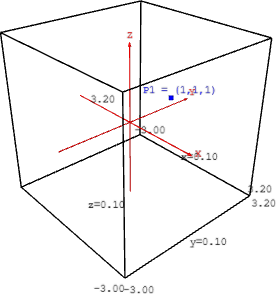
\includegraphics[height=0.6\textheight]{projective-plane-01.png}}
\end{figure}
\end{frame}
\note{Let's consider an affine space. Let's mark a single point with coordinates (1,1,1).}

\begin{frame}{Projective plane -- $\mathbf{P}^2$}
\begin{figure}
    \centering
    \href{https://doktor-ziel.github.io/ECC/projective-plane-02.html}{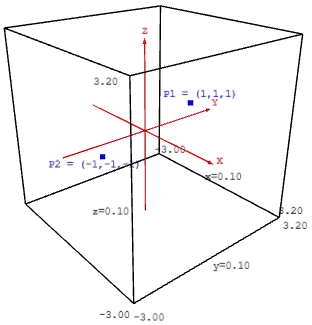
\includegraphics[height=0.6\textheight]{projective-plane-02.png}}
\end{figure}
\end{frame}

\note{Let's mark another point in affine space. Its coordinates are (-1,-1,-1). According to the previous definition, they both are in relation I defined earlier (because they are laying on one line going through the origin of coordinate system}

\begin{frame}{Projective plane -- $\mathbf{P}^2$}
\begin{figure}
    \centering
    \href{https://doktor-ziel.github.io/ECC/projective-plane-03.html}{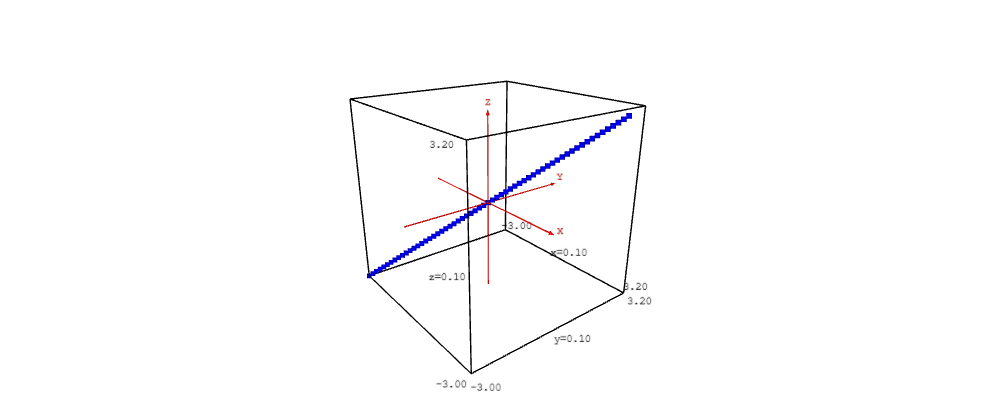
\includegraphics[height=0.6\textheight]{projective-plane-03.png}}
\end{figure}
\end{frame}

\note{In fact any of two points laying on this line are in relation with each other (of course without origin itself). Mathematically speaking, all those points form equivalence class of the relation we keep talking about. We can define infinitely many such classes of equivalence (because there are infinitely many lines going through origin of coordinates system. Each equivalence class is one element of projective space.

Note that affine space and projective space are related. We define $n$ dimensional projective space for $n+1$ dimensional affine space. Because we are considering three dimensional affine space, we've just defined two dimensional projective space. If space has two dimensions, we call it plane. So we defined projective plane.

We need to present elements of that plane much easier than that.
}

\begin{frame}{Projective plane -- $\mathbf{P}^2$}
\begin{figure}
    \centering
    \href{https://doktor-ziel.github.io/ECC/projective-plane-04.html}{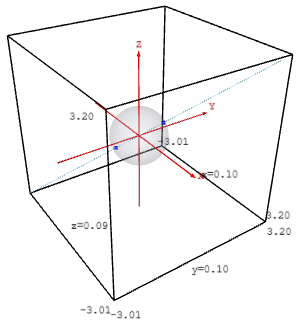
\includegraphics[height=0.4\textheight]{projective-plane-04.png}}
\end{figure}
\end{frame}

\note{It's very common that we draw points of projective plane as points of intersection the line and unit sphere. It's quite important that we mark two points in affine space as one point in projective space.}

\begin{frame}{Projective plane -- $\mathbf{P}^2$}
\begin{figure}
    \centering
    \href{https://doktor-ziel.github.io/ECC/projective-plane-05.html}{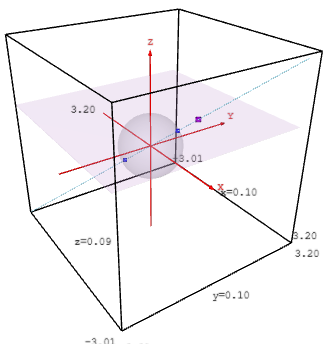
\includegraphics[height=0.6\textheight]{projective-plane-05.png}}
\end{figure}
\end{frame}

\note{We are not used to consider geometry on sphere. So we would like to present projective plane in affine plane. One of method is "projection" of point on chosen plane - the most common is choosing plane with z coordinate equal to one. Very poetically speaking, we can imagine that there is a candle in the centre of the sphere. And we observe the shadow of points on the wall. 
This approach has big disadvantage. We cannot see all points of projective plane that way. We cannot see any point with z coordinate equal to 0}

\begin{frame}{Projective plane -- $\mathbf{P}^2$}
\begin{figure}
    \centering
    \href{https://doktor-ziel.github.io/ECC/projective-plane-06.html}{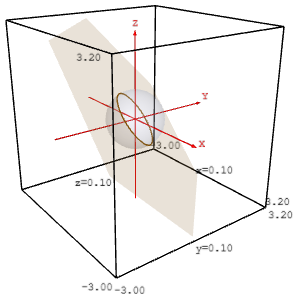
\includegraphics[height=0.6\textheight]{projective-plane-06.png}}
\end{figure}
\end{frame}

\note{Let's consider the line in projective space. In general - line is set of points laying in the straight line. We said that line in affine space defines point in projective plane. Hence the plane in affine space defines the line in projective plane. And it makes perfect sense. If we mark intersections of plane and unit sphere, we observe a line on this sphere - it something like equator }

\begin{frame}{Projective plane -- $\mathbf{P}^2$}
\begin{figure}
    \centering
    \href{https://doktor-ziel.github.io/ECC/projective-plane-07.html}{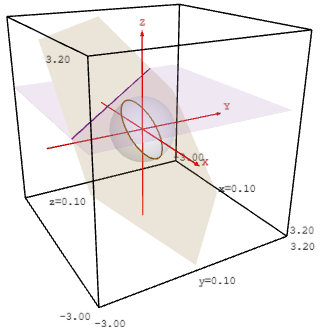
\includegraphics[height=0.6\textheight]{projective-plane-07.png}}
\end{figure}
\end{frame}

\note{Moreover, if we project this line on plane z=1, we will observe line.}

\begin{frame}{Projective plane -- $\mathbf{P}^2$}
\begin{figure}
    \centering
    \href{https://doktor-ziel.github.io/ECC/projective-plane-08.html}{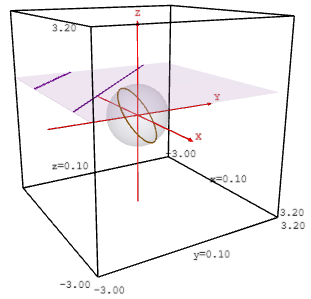
\includegraphics[height=0.6\textheight]{projective-plane-08.png}}
\end{figure}
\end{frame}

\note{Let's consider another parallel line in plane z=1.}

\begin{frame}{Projective plane -- $\mathbf{P}^2$}
\begin{figure}
    \centering
    \href{https://doktor-ziel.github.io/ECC/projective-plane-09.html}{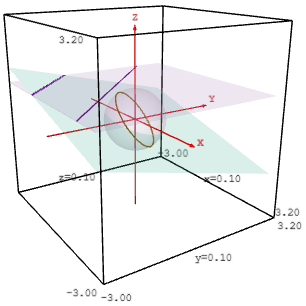
\includegraphics[height=0.6\textheight]{projective-plane-09.png}}
\end{figure}
\end{frame}

\note{We can define only one plane containing this line and the origin of coordinates system. }

\begin{frame}{Projective plane -- $\mathbf{P}^2$}
\begin{figure}
    \centering
    \href{https://doktor-ziel.github.io/ECC/projective-plane-10.html}{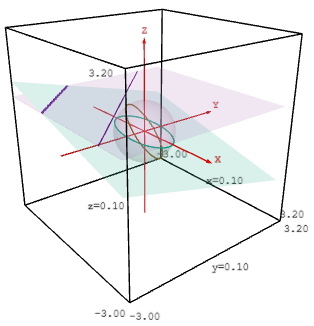
\includegraphics[height=0.6\textheight]{projective-plane-10.png}}
\end{figure}
\end{frame}

\note{Hence, this second line is projection of another equator of the unit sphere.}

\begin{frame}{Projective plane -- $\mathbf{P}^2$}
\begin{figure}
    \centering
    \href{https://doktor-ziel.github.io/ECC/projective-plane-11.html}{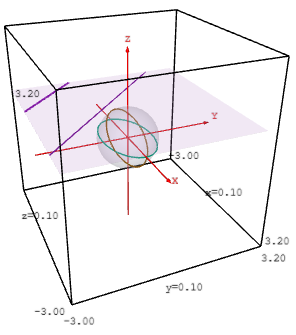
\includegraphics[height=0.6\textheight]{projective-plane-11.png}}
\end{figure}
\end{frame}

\note{Observe that two parallel lines in the affine space have common point in projective plane. This common point is example of the point which cannot be marked in affine space. We call it point in infinity.}

\begin{frame}{}
\begin{figure}
    \centering
    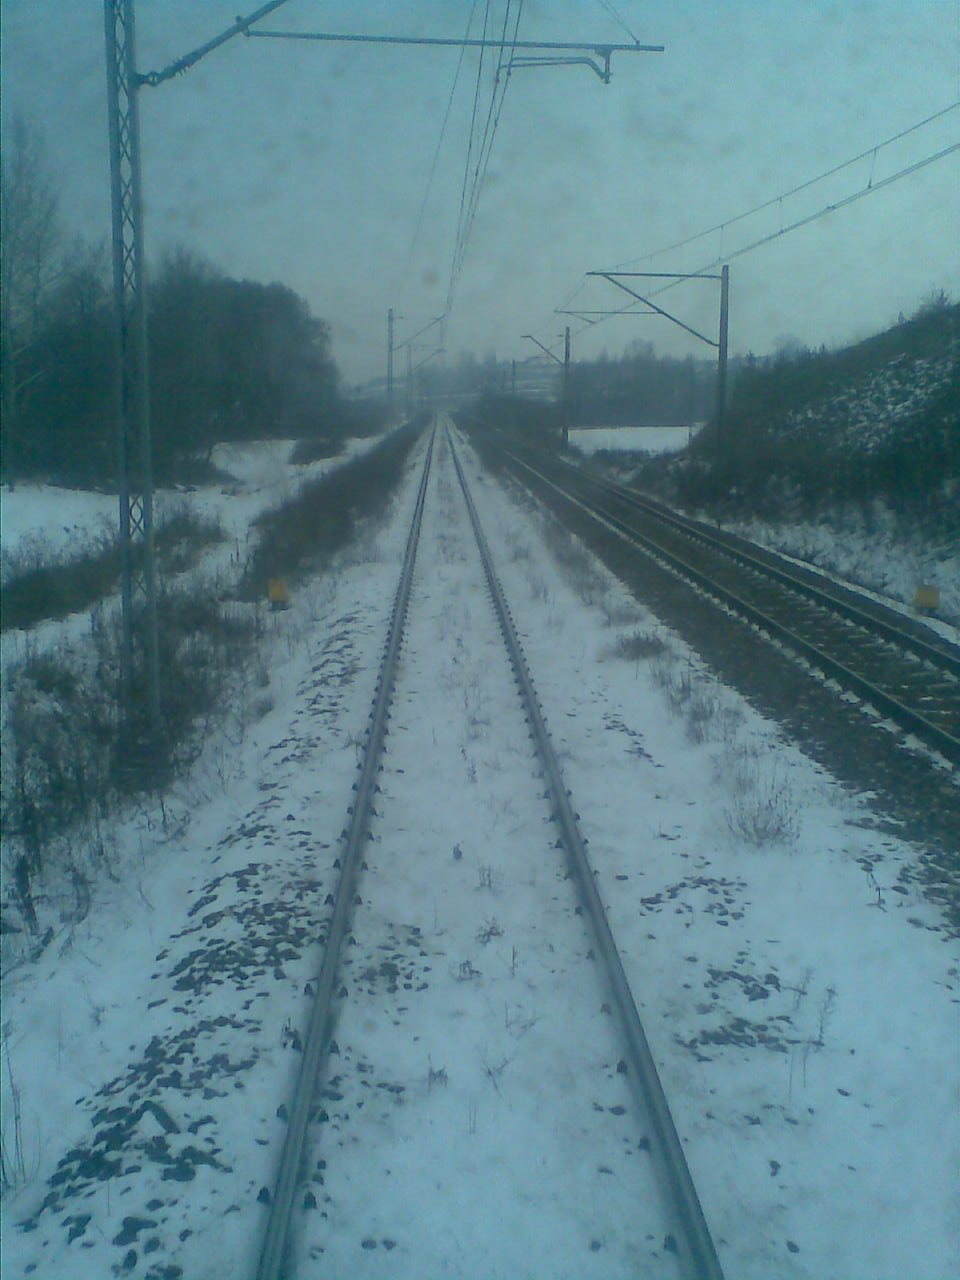
\includegraphics[height=0.9\textheight]{track.jpg}
\end{figure}
\end{frame}

\note{Just think, is it really so strange that two parallel lines intersect in infinity?}

\section{Elliptic curves: definition}

\begin{frame}{Elliptic curve}
\begin{definition}
    Cubic curve is an algebraic curve defined by a homogeneous polynomial of degree 3 in projective plane.
\end{definition}
\begin{definition}
    Elliptic curve is a smooth cubic curve with one chosen point (\textit{infinity point})
\end{definition}
\end{frame}

\note{I hope you are not sick of this mathematical formalism. It's the most important part of everything I was talking about: we define elliptic curves in projective plane. And that's why they have so many useful properties.

What means homogeneous polynomial? In such a polynomial every monomial has the same degree. In case of elliptic curve this degree is equal to three.}

\begin{frame}{Weierstrass equation}
$$y^2z + a_1xyz + a_3yz^2 = x^3 + a_2x^2 z~+ a_4xz^2+a_6z^3$$
\end{frame}

\note{Every elliptic curve can be described by Weierstrass formula. And as you can see all terms have degree equal to three.}


\begin{frame}{Weierstrass equation - simplification}
$$y^2z = x^3 + Axz^2 + Bz^3$$
where 
$$\Delta = -16(4A^3 + 27B^2) \neq 0$$
\end{frame}

\note{That formula can be simplified in many situations.}

\begin{frame}{Example elliptic curve}
    \begin{figure}
        \centering
        \href{https://doktor-ziel.github.io/ECC/elliptic-curve-00.html}{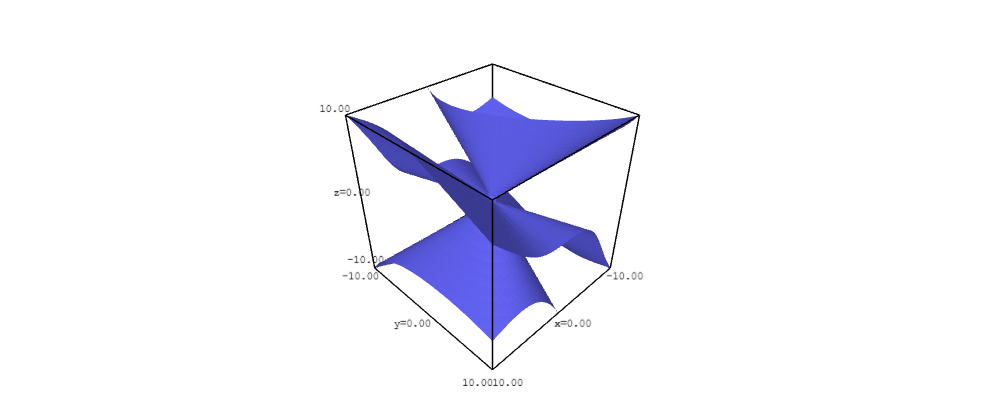
\includegraphics[height=0.7\textheight]{elliptic-curve-00.png}}
        \caption{$y^2z + yz^2 = x^3 + x^2z - 2xz^2$}
    \end{figure}
\end{frame}

\note{If we mark all points in affine space satisfying that formula we obtain three surfaces}

\begin{frame}{Example elliptic curve}
    \begin{figure}
        \centering
        \href{https://doktor-ziel.github.io/ECC/elliptic-curve-01.html}{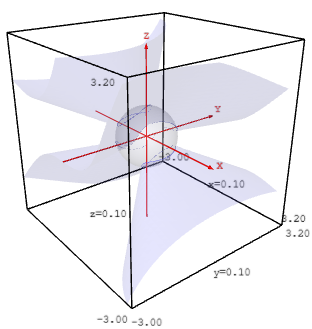
\includegraphics[height=0.8\textheight]{elliptic-curve-01.png}}
    \end{figure}
\end{frame}

\note{But we want to see that curve in projective plane.}

\begin{frame}{Example elliptic curve}
    \begin{figure}
        \centering
        \href{https://doktor-ziel.github.io/ECC/elliptic-curve-02.html}{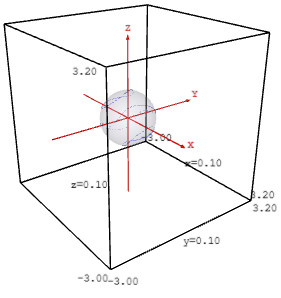
\includegraphics[height=0.8\textheight]{elliptic-curve-02.png}}
    \end{figure}
\end{frame}

\note{And as you can see, we have quite nice curve in the surface of unit sphere.}

\begin{frame}{Example elliptic curve}
    \begin{figure}
        \centering
        \href{https://doktor-ziel.github.io/ECC/elliptic-curve-03.html}{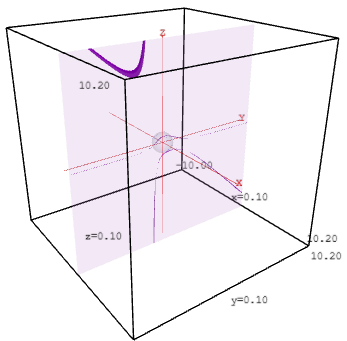
\includegraphics[height=0.8\textheight]{elliptic-curve-03.png}}
    \end{figure}
\end{frame}


\note{We can project this curve onto three main planes. Firstly, we have plane x=1}

\begin{frame}{Example elliptic curve}
    \begin{figure}
        \centering
        \href{https://doktor-ziel.github.io/ECC/elliptic-curve-04.html}{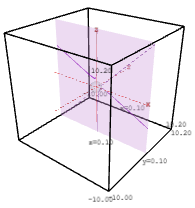
\includegraphics[height=0.8\textheight]{elliptic-curve-04.png}}
    \end{figure}
\end{frame}

\note{Now, we have plane y=1}

\begin{frame}{Example elliptic curve}
    \begin{figure}
        \centering
        \href{https://doktor-ziel.github.io/ECC/elliptic-curve-05.html}{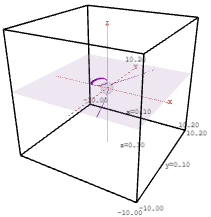
\includegraphics[height=0.8\textheight]{elliptic-curve-05.png}}
    \end{figure}
\end{frame}

\note{And finally, the plane $z=1$. I think, many of you could see this one plot. I think this is the most common way of presenting the elliptic curve.}

\begin{frame}{Example elliptic curve}
    \begin{figure}
        \centering
        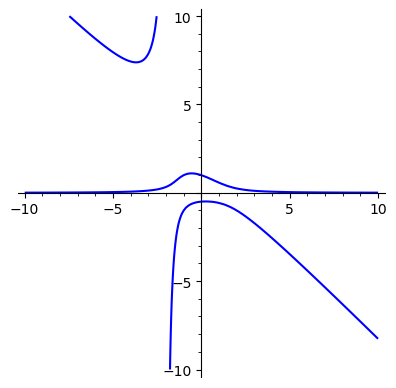
\includegraphics[height=0.8\textheight]{elliptic-curve-06.png}
    \end{figure}
\end{frame}


\note{And just projections once more.}

\begin{frame}{Example elliptic curve}
    \begin{figure}
        \centering
        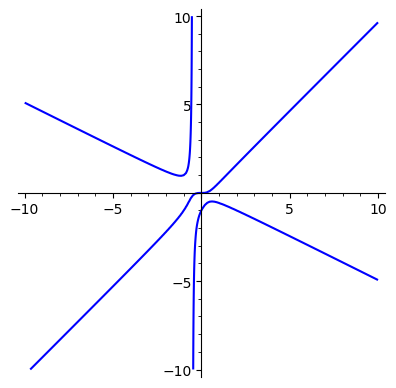
\includegraphics[height=0.8\textheight]{elliptic-curve-07.png}
    \end{figure}
\end{frame}

\begin{frame}{Example elliptic curve}
    \begin{figure}
        \centering
        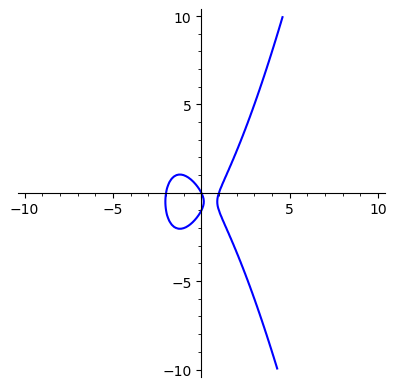
\includegraphics[height=0.8\textheight]{elliptic-curve-08.png}
    \end{figure}
\end{frame}

\begin{frame}{More examples}
    \begin{figure}
        \centering
        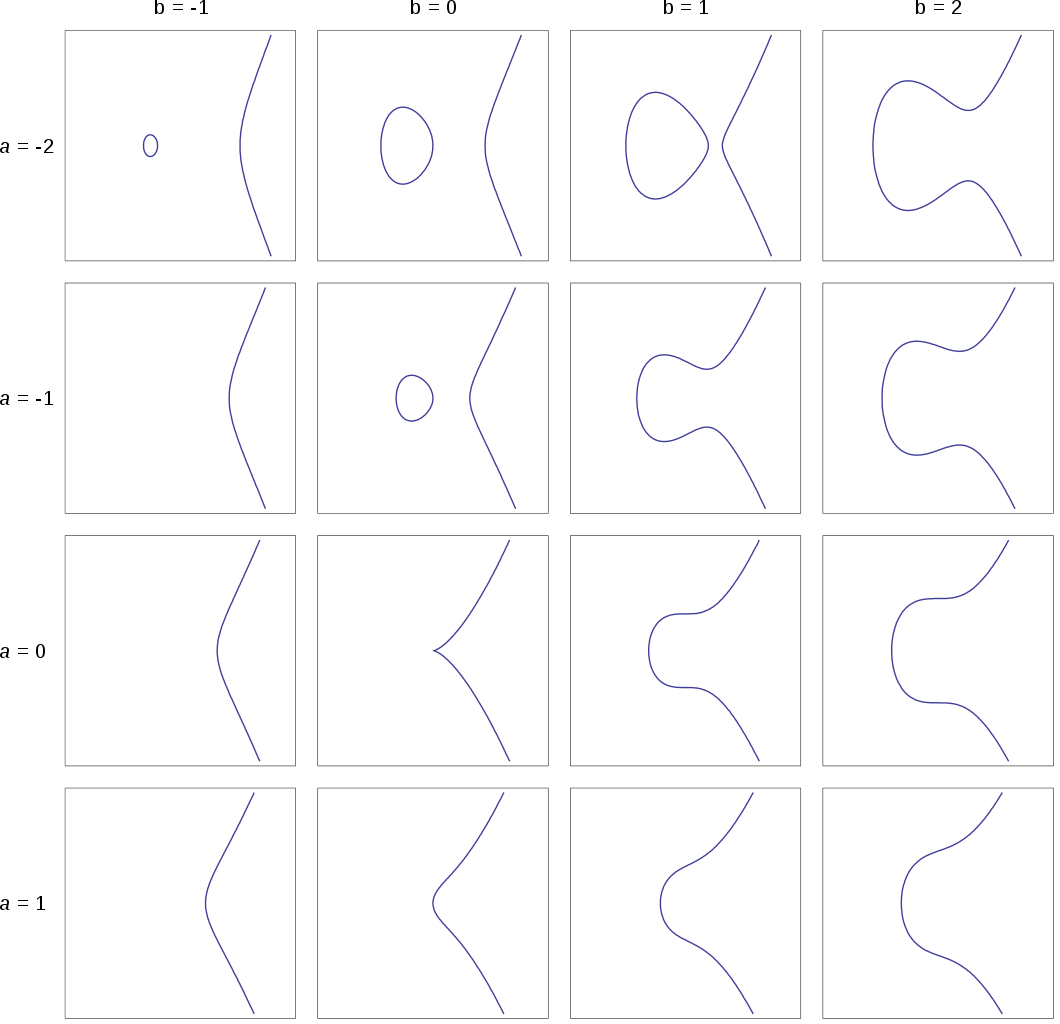
\includegraphics[height=0.7\textheight]{elliptic-curves.png}
        \caption{Source: \cite{wiki:elliptic:curve}}
    \end{figure}
\end{frame}

\note{Before we move to adding points, some examples of possible shapes of projection of elliptic curves onto plane $z=1$}

\section{Elliptic curves: adding points}

\begin{frame}{Adding points}
    \begin{figure}
        \centering
        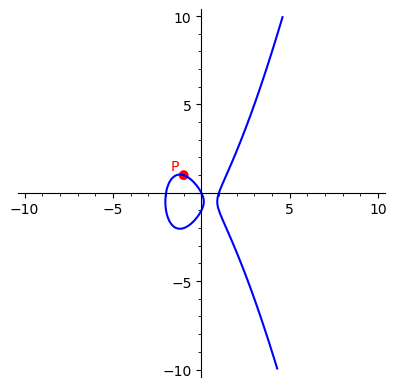
\includegraphics[height=0.7\textheight]{adding-points-01.png}
        \caption{$y^2 + y = x^3 + x^2 - 2x$, $P=(-1,1)$}
    \end{figure}
\end{frame}

\note{We want to add two points laying on the curve. Let note the first one as $P$}

\begin{frame}{Adding points}
    \begin{figure}
        \centering
        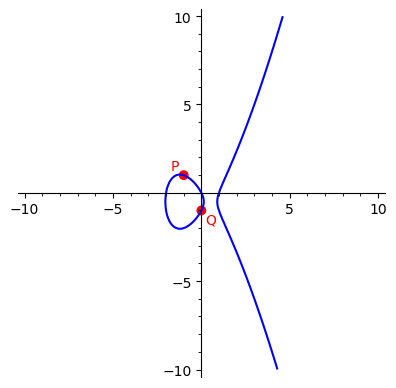
\includegraphics[height=0.7\textheight]{adding-points-02.png}
        \caption{$y^2 + y = x^3 + x^2 - 2x$, $P=(-1,1)$, $Q=(0,-1)$}
    \end{figure}
\end{frame}

\note{The other one is $Q$}


\begin{frame}{Adding points}
    \begin{figure}
        \centering
        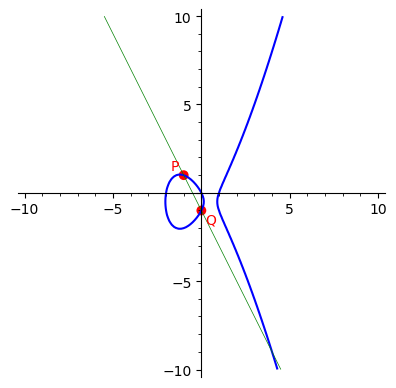
\includegraphics[height=0.7\textheight]{adding-points-03.png}
        \caption{$y^2 + y = x^3 + x^2 - 2x$, $P=(-1,1)$, $Q=(0,-1)$}
    \end{figure}
\end{frame}

\note{We draw line going through those two points. Because elliptic curve is defined in projective plane, we are sure that there is third point of intersection of this line and curve. }

\begin{frame}{Adding points}
    \begin{figure}
        \centering
        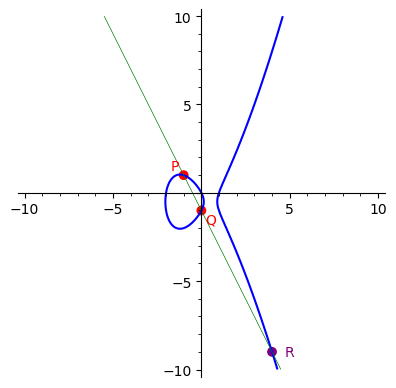
\includegraphics[height=0.7\textheight]{adding-points-04.png}
        \caption{$y^2 + y = x^3 + x^2 - 2x$, $P=(-1,1)$, $Q=(0,-1)$, $R=(4,-9)$}
    \end{figure}
\end{frame}

\note{Let's denote it by $R$}

\begin{frame}{Adding points}
    \begin{figure}
        \centering
        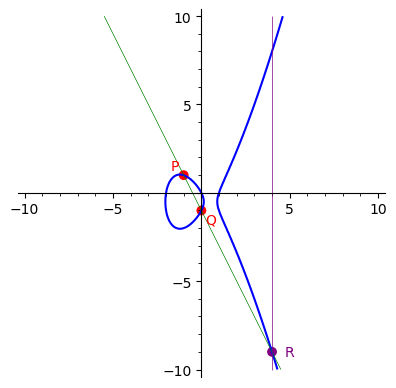
\includegraphics[height=0.7\textheight]{adding-points-05.png}
        \caption{$y^2 + y = x^3 + x^2 - 2x$, $P=(-1,1)$, $Q=(0,-1)$, $R=(4,-9)$}
    \end{figure}
\end{frame}

\note{Now we draw line going through point $R$ and point in infinity. In practice it is line parallel to $OY$ axis. And again, there is exactly one more point of intersection the line and the curve.}

\begin{frame}{Adding points}
    \begin{figure}
        \centering
        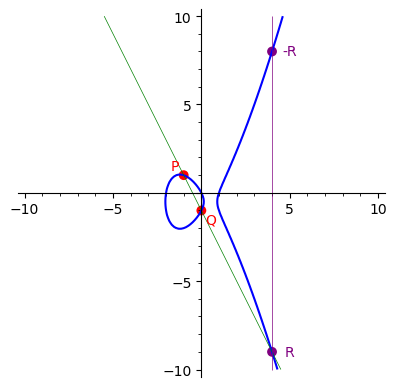
\includegraphics[height=0.7\textheight]{adding-points-06.png}
        \caption{$y^2 + y = x^3 + x^2 - 2x$, $P=(-1,1)$, $Q=(0,-1)$, $R=(4,-9)$}
    \end{figure}
\end{frame}

\note{Let's denote this point by $-R$. And it's in fact the inverse of point $R$ from algebraic point of view.}

\begin{frame}{Adding points}
    \begin{figure}
        \centering
        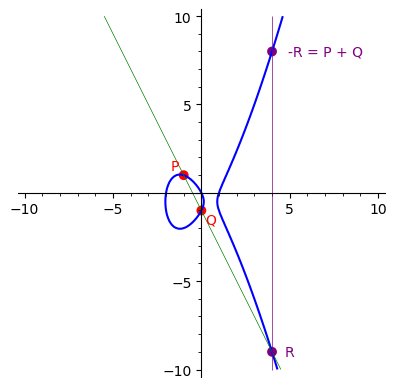
\includegraphics[height=0.7\textheight]{adding-points-07.png}
        \caption{$y^2 + y = x^3 + x^2 - 2x$, $P=(-1,1)$, $Q=(0,-1)$, $R=(4,-9)$, $-R=(4,8)$}
    \end{figure}
\end{frame}

\note{This point $-R$ is result of adding $P$ and $Q$}

\section{Elliptic curve cryptography}

\begin{frame}{Elliptic curves Diffie-Hellman algorithm}
    \begin{itemize}
    \item Alice and Bob want to establish secret key for AES algorithm
    \item They publicly agree to use some elliptic curve $E$ over finite field $K$
    \item They publicly agree to use point $P$ of curve $E$
\end{itemize}
\end{frame}

\note{Adding points of elliptic curve and its properties are essential for using curves in cryptography. Let me show you very simple algorithm used for establishing secret key safe communication}

\begin{frame}{Elliptic curves Diffie-Hellman algorithm}
\begin{columns}
    \begin{column}{0.5\textwidth}
        \centerline{\textbf{Alice}}
        \begin{enumerate}
            \item Chooses private key $a$
            \item Calculates public key $K_A = a \cdot P$
            \item Sends the public key to Bob
            \item Receives the public key from Bob $K_B$
            \item Calculates the final key:
            $$K = a \cdot K_B = a\cdot b \cdot P$$
        \end{enumerate}
    \end{column}
    \begin{column}{0.5\textwidth}
        \centerline{\textbf{Bob}}
        \begin{enumerate}
            \item Chooses private key $b$
            \item Calculates public key $K_B = b \cdot P$
            \item Sends the public key to Alice
            \item Receives the public key from Alice $K_A$
            \item Calculates the final key:
            $$K =  b \cdot K_A = a \cdot b \cdot P$$
        \end{enumerate}
    \end{column}
\end{columns}
\end{frame}


\begin{frame}{TLS}
    \begin{figure}
        \centering
        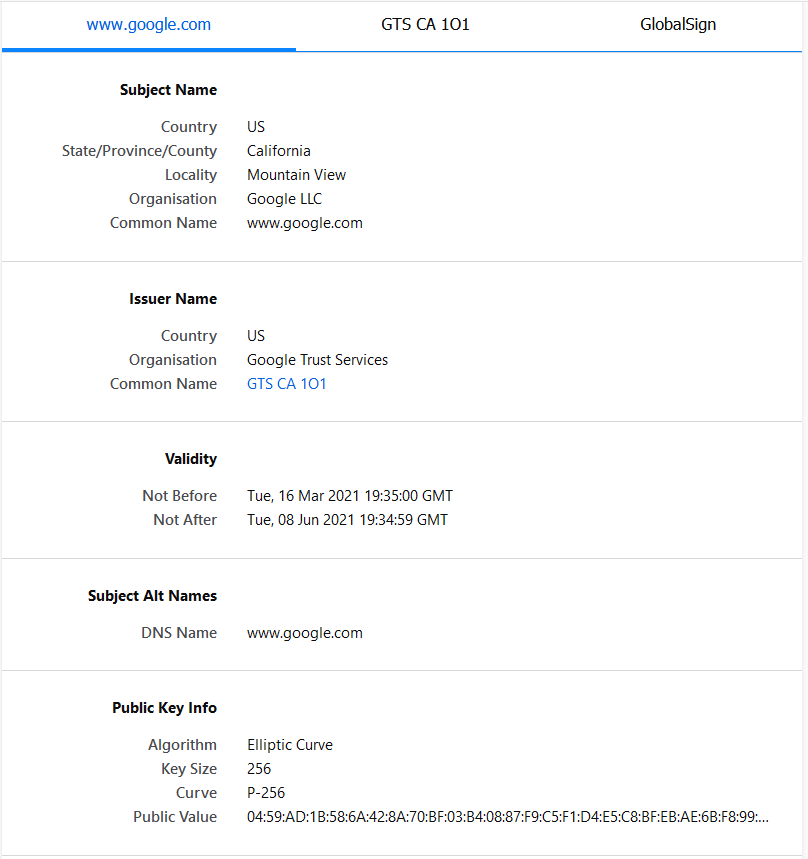
\includegraphics[height=0.8\textheight]{ssl-01.PNG}
    \end{figure}
\end{frame}

\note{ECC is widely used in modern Internet. Just see the TLS certificate of google.com. This certificate contains the public key for ECC asymmetric cryptography.}

\section{Conclusion}

\begin{frame}{Conclusion}
\begin{figure}
    \centering
    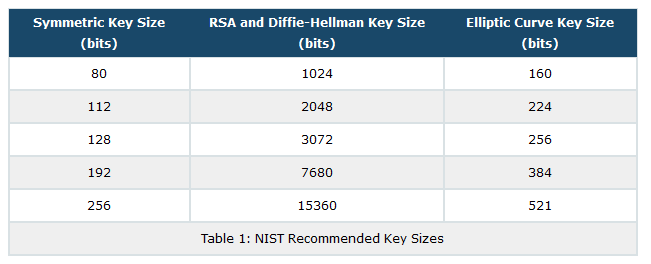
\includegraphics[width=0.9\textwidth]{summary-01.PNG}
\end{figure}
\end{frame}

\note{To conclude my presentation I'd like to emphasise that ECC is used. And NIST claims that ECC gives the same level of security like other asymmetric algorithms using much shorter keys. Hence computer needs shorter time to secure our documents using ECC than traditional cryptography. }

\begin{frame}{Conclusion}
\begin{figure}
    \centering
    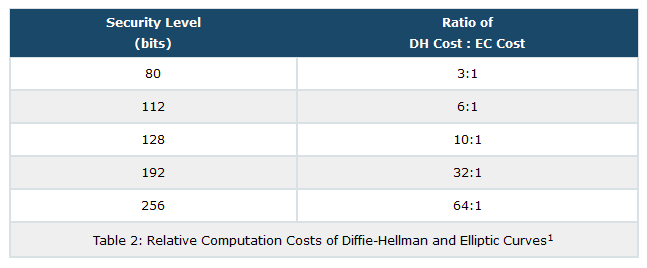
\includegraphics[width=0.9\textwidth]{summary-02.PNG}
\end{figure}
    
\end{frame}

\setbeamertemplate{bibliography item}{\insertbiblabel}
\begin{frame}{References}
    \footnotesize{
        \begin{thebibliography}{99}
            \bibitem{wiki:diffie:hellman} \href{https://en.wikipedia.org/wiki/Diffie\%E2\%80\%93Hellman_key_exchange}{Diffie-Hellman key exchange - Wikipedia}
            \bibitem{wiki:elliptic:curve} \href{https://en.wikipedia.org/wiki/Elliptic_curve}{Elliptic curve - Wikipedia}
            \bibitem{nsa:elliptic:curve} \href{https://web.archive.org/web/20130918005527/http://www.nsa.gov/business/programs/elliptic_curve.shtml}{NSA about elliptic curves cryptography}
        \end{thebibliography}
    }
\end{frame}

\end{document}